
\begin{theappendices}

\chapter{Experimental Equipment}

\begin{table}[h!]
\caption[]{Survey Data}
\begin{tabular}{|L{0.2\textwidth}|L{0.2\textwidth}|}
\hline
\textbf{Headings} & \textbf{Data} \\ \hline
Yes               & 50\%          \\ \hline
No                & 50\%          \\ \hline
\end{tabular}
\end{table}

\vspace{\baselineskip}
\begin{table}[h!]
\caption[]{More Survey Data}
\begin{tabular}{|L{0.2\textwidth}|L{0.2\textwidth}|}
\hline
\textbf{Headings} & \textbf{Data} \\ \hline
Yes               & 20\%          \\ \hline
No                & 80\%          \\ \hline
\end{tabular}
\end{table}
\vspace{\baselineskip}

\chapter{The Second Appendix}

\begin{figure}[htb!]
    \caption[]{Scattergraph Chart}
    
    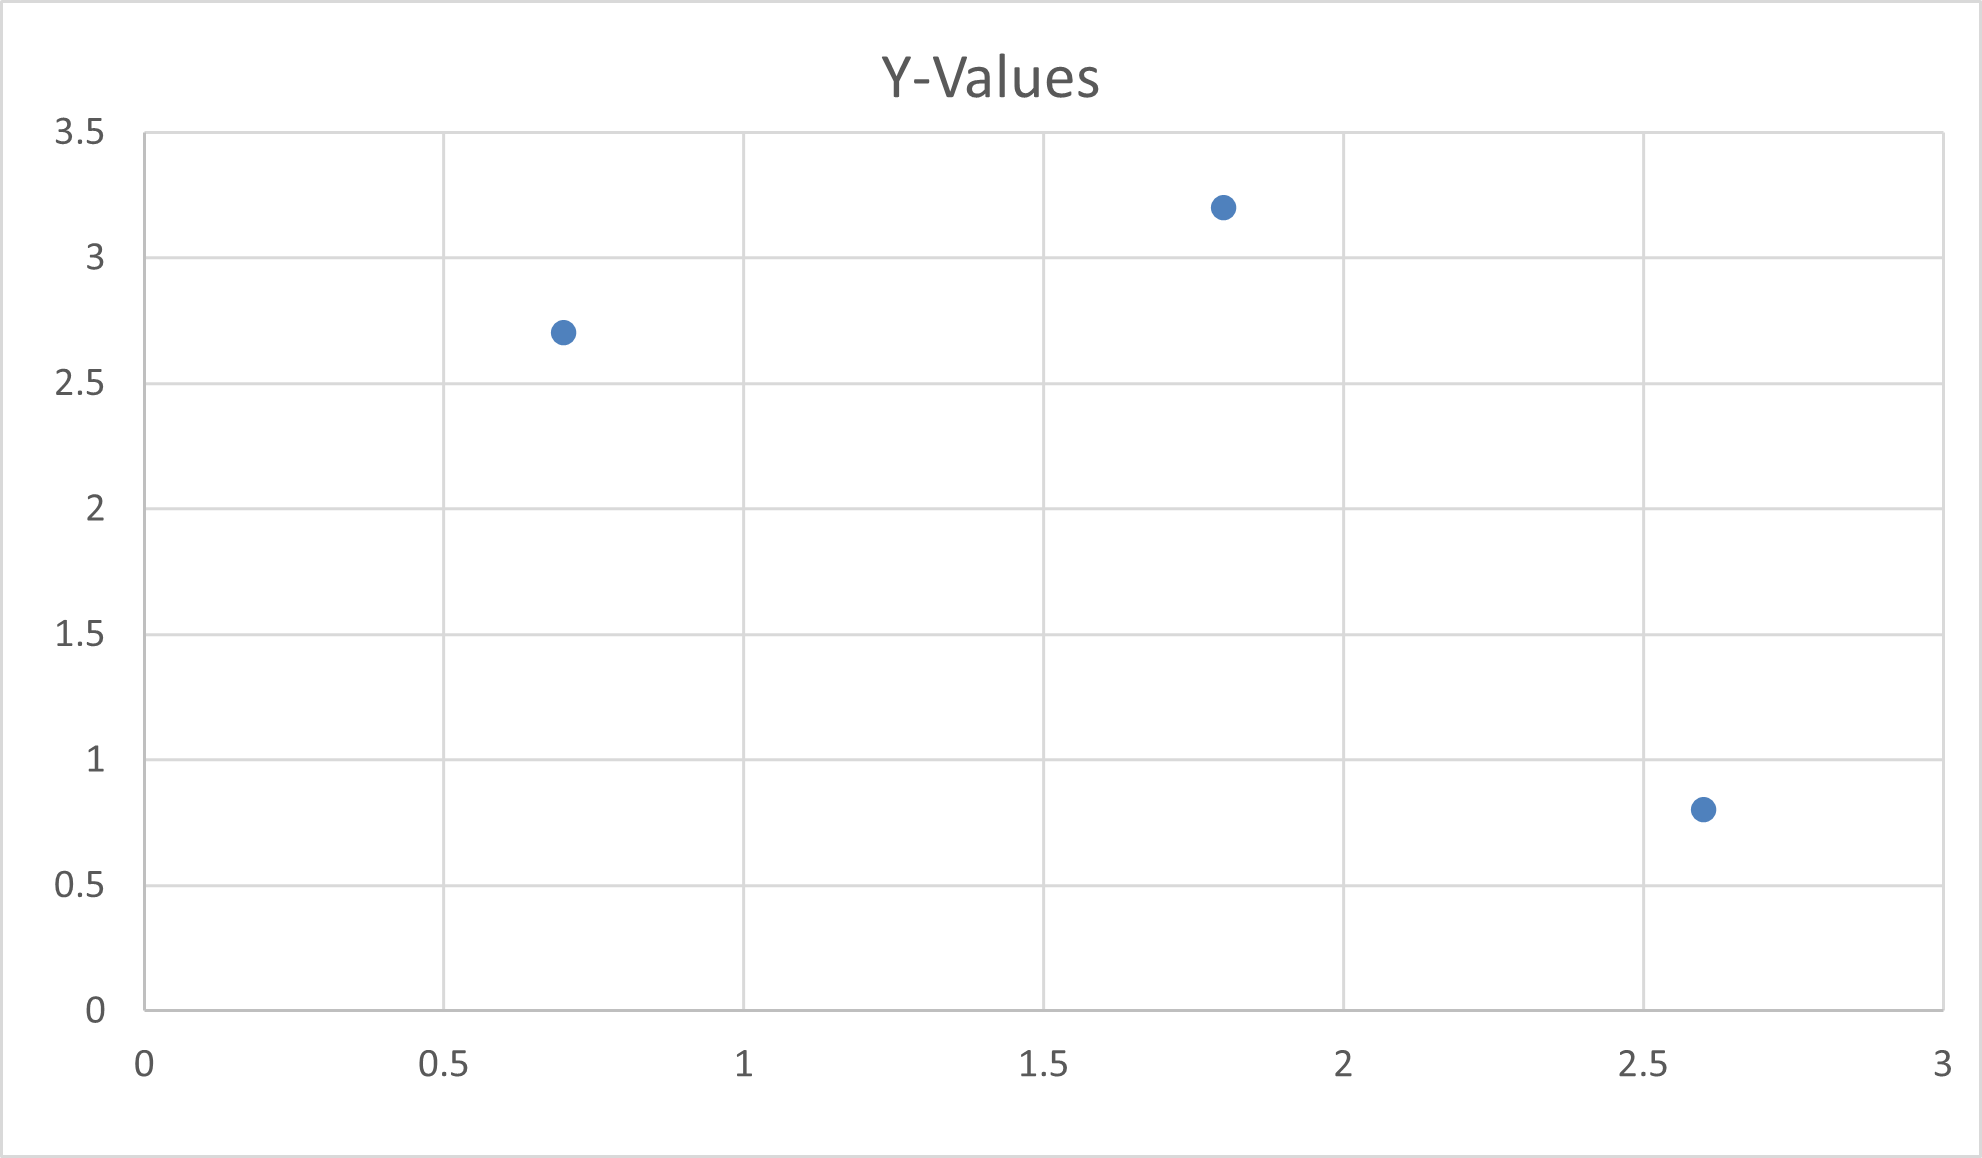
\includegraphics[width = 0.9\textwidth]{Figures/graph.png}
    \label{fig:graph}
\end{figure}
\FloatBarrier

\end{theappendices}